\documentclass{article}
\usepackage[utf8]{inputenc}
\usepackage{csquotes}
\usepackage[textsize=footnotesize]{todonotes}
\usepackage{subcaption}
% \usepackage{url}
\PassOptionsToPackage{hyphens}{url}\usepackage{hyperref}


\urlstyle{same}

\setlength{\parindent}{0pt}

\begin{document}

Dear Reviewer,

\vspace{0.25in}

Thank you for considering our manuscript for publication and for providing constructive feedback.
Hereunder you will find our detailed replies to all Your comments.
The changes are highlighted in the output of the latexdiff file attached to this cover letter.


\section{Reviewer 1}

\paragraph{Issue 0:}
\begin{displayquote}
In truth, the purpose of the work is not precisely defined. Reading the article, one has the impression that one will take an ECG signal, apply a wavelet transform to de-noise the signal, then count the STFT to get a spectrogram and finally apply a CNN to classify the signal with and without heart disease. To do this using the well-known tools available in python. Where is the novelty here?
\end{displayquote}

\paragraph{Answer:}
Thank you for this issue. The novelty in proposed work is representation of data to convolutional neural network model in well understood i.e., Spectrograms. Moreover,  frequency filtration was applied through STFT with purpose of reducing data at possible limit at which a simple architecture of CNN model showed high accuracy rather than to utilize the complex model which ultimately requires more momeory and computational power.\\\\

Because the novelty wast not stated explicitly in the text, we modified 'Introduction' section adding '\textit{The novelty of proposed work is representation of data to convolutional neural net-work model in well-defined form i.e., Spectrograms. Additionally, data size reduction aim is achieved through frequency filtration at which a simple architecture of CNN model showed high accuracy rather than to utilize the complex model which ulti-mately requires more memory and computational power.}' in lines 125-129.

\paragraph{Issue 1:}
\begin{displayquote}
The work concerns the classification of ECG signals, and in particular "Anteroseptal myocardial infarction (ASMI) considered in this study is one of the life-threatening heart diseases that occurs due to the rupture of the volatile atherosclerotic plaque in the left anterior descending artery [3]." In the entire paper, there is not a single example of an ECG signal waveform with this cardiovascular disease, nor is it shown how the spectrogram of the ECG signal differs between a healthy person and one with ASMI or other cardiovascular disease.
\end{displayquote}

\paragraph{Answer:}
Thank you for this issue. Lead V1 data was considered for the ECG signals to differentiate between NORMAL and ASMI sample. The difference can be find in the base of the signals. As asked, the ECG signals and Spectrogram of both cateogories are presented in below figure. One can see a difference between NORM and ASMI spectorgram at signal base. The shadow is spreaded in ASMI spectrogram while it is condensed in NORMAL spectrogram.
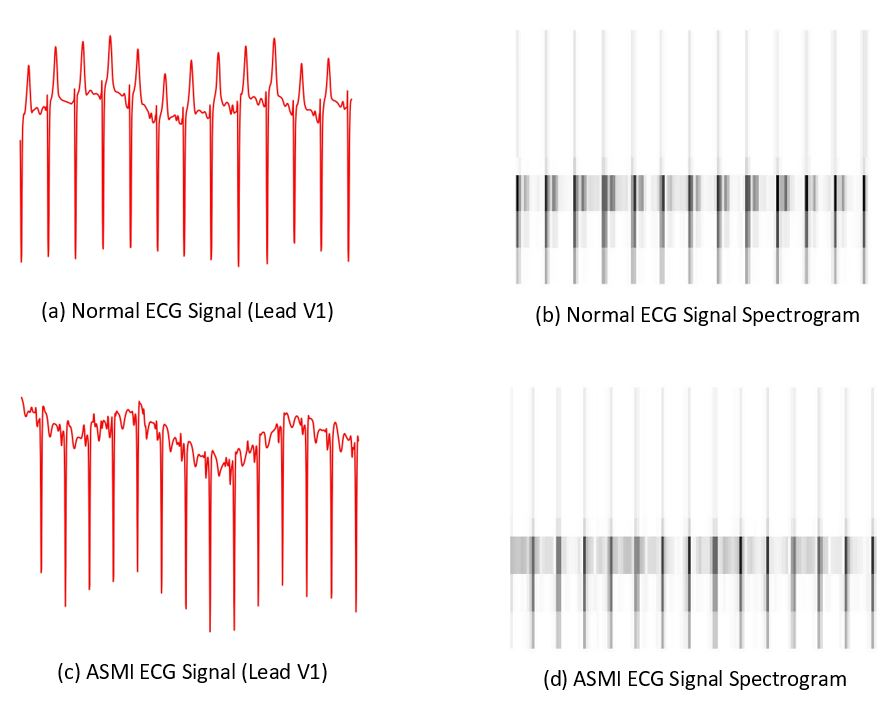
\includegraphics[scale=0.55]{Signal and spectrogram img.JPG}
\\\\
Since there was not a spectrogram example given in the article so we added a figure (Fig. 1) in 'Introduction' section with the following text \textit{`In the below fig. 2, (a) and (c) are showing the raw signal of NORM and ASMI class respectively, while (b) and (d) represents the transformation into spectrograms for both classes. A difference can be seen between NORM and ASMI spectrogram at signal base. There is a spread or light shadow in ASMI spectrogram which is condensed or dark in NORM spectrogram.'} in lines 102-106

\paragraph{Issue 2:}
\begin{displayquote}
 The Short Time Fourier Transform (STFT) is one of the time-frequency transformation method existing in the signal processing. What other time-frequency transform methods have been considered?
\end{displayquote}

\paragraph{Answer:}
Thanks for asking. In this study, STFT is used for time-frequency transformation because it is comparatively faster and has good precision as highlighted in [46]. The other possible time-frequency transformation methods are Fast Fourier Transformation [45], synchrosqueezed transform [46] and  Continuous Wavelet Transformation [47]. \\\\
‌
Because we utilized STFT only therefore we added one line in the `introduction' section adding '\textit{STFT is comparatively faster and has good precision as highlighted in [46]. The other possible time-frequency transformation methods are Fast Fourier Transformation [45], synchro squeezed transform [46] and Continuous Wavelet Transformation [47].'} at lines 92-95

\paragraph{Issue 3:}
\begin{displayquote}
Quite a few modern (recently published) methods of noise reducing in the ECG signal have been presented, so why was the wavelet transform used, which has been known for more than a dozen years and is known not to work effectively in all cases, which is important when analyzing ECG signals with heart disease.
\end{displayquote}

\paragraph{Answer:}
Thank you for raising this issue. The main reason for preference of wavelet transformation for signal denoising is that it offers range of wavelets i.e., db, haar, coif, sym and bior. Therefore, there are number of options available under single approach to find the best matching wavelet for the presented problem. \\\\

The reason is given in section `introduction` adding '\textit{The main reason for preference of WT for signal denoising is that it offers range of wavelets i.e., Daubechies, Haar, Coif, Sym and Bior. Therefore, there are number of op-tions available under single approach to find the best matching wavelet for the pre-sented problem.}' at lines 84-87

\paragraph{Issue 4:}
\begin{displayquote}
Section 3.1.2 "Frequency Filtration". There is a lack of mathematical formulas for the steps involved in implementing the proposed algorithm. There is a description of the algorithm (Algorithm 2), but it is insufficient for a correct representation of the filtration. Why is the Sampling Frequency  value calculated in step 3? Is it a different frequency than the one at which the signal was recorded? In the next step (del (...)) the numeric value of 2 was used. Where does this value come from? What is its meaning? This operation suggests cutting all frequency components above a certain frequency value in the frequency spectrum. It is worth showing the frequency spectrum of the analyzed signal after such an operation and the signal in the time domain. How does this operation affect the spectrograms obtained later (by STFT)? This operation suggests cutting all frequency components above a certain frequency value in the frequency spectrum. It is worth showing the frequency spectrum of the analyzed signal after such an operation and the signal in the time domain. How does this operation affect the spectrograms obtained later (by STFT)?
\end{displayquote}

\paragraph{Issue 4a:}
\begin{displayquote}
Section 3.1.2 "Frequency Filtration". There is a lack of mathematical formulas for the steps involved in implementing the proposed algorithm. There is a description of the algorithm (Algorithm 2), but it is insufficient for a correct representation of the filtration. Why is the Sampling Frequency  value calculated in step 3? Is it a different frequency than the one at which the signal was recorded? In the next step (del (...)) the numeric value of 2 was used. Where does this value come from? What is its meaning? This operation suggests cutting all frequency components above a certain frequency value in the frequency spectrum. It is worth showing the frequency spectrum of the analyzed signal after such an operation and the signal in the time domain. How does this operation affect the spectrograms obtained later (by STFT)?
\end{displayquote}

\paragraph{Answer:}
Thank you for this issue. The signal was decompose into time-frequency domain and then corresponding frequencies were calculated through the sampling frequency  which were used in the next stage to apply the threshold for frequency filtration.  As mentioned, the said sampling frequency is not different than at which signal was recorded but it is a type of variable in which corresponding frequencies were saved. Since, one of the study aim was to reduce the data, therefore, by analysing ECG signals visually and by experiments we set the threshold of 2 which means all the data points associated with frequency more than two i.e., high QRS peaks (downward in lead V1) will be discard because the signals can classify through the base patterns.

\paragraph{Issue 4b:}
\begin{displayquote}
"Frequency Filtration". This operation suggests cutting all frequency components above a certain frequency value in the frequency spectrum. It is worth showing the frequency spectrum of the analyzed signal after such an operation and the signal in the time domain. How does this operation affect the spectrograms obtained later (by STFT)?
\end{displayquote}
\paragraph{Answer:}
Thank you for this issue. The figure has been added.\\\\
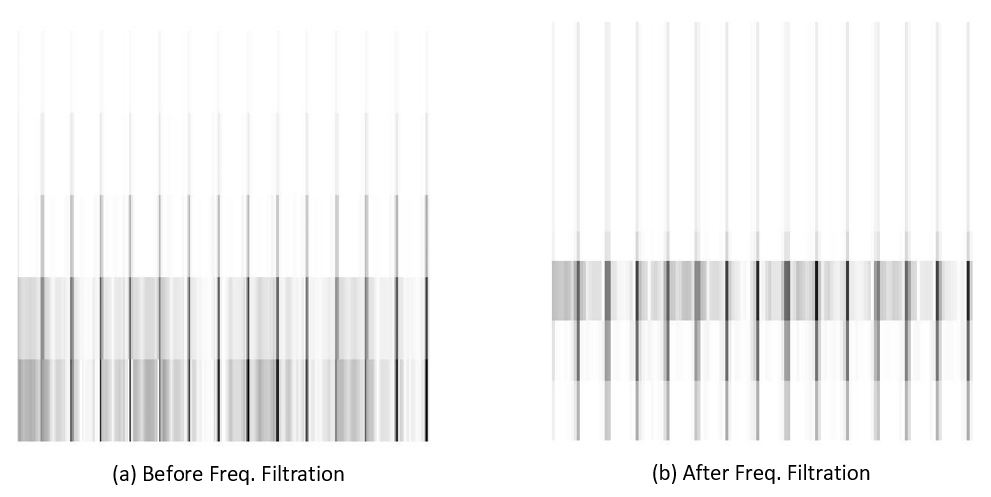
\includegraphics[scale=0.5]{before and after spectrogram.JPG}\\
In the above figure, (a) is showing spectrogram before frequency filtration while (b) is showing after operation. One can see the black shadow reduced in fig (b) due to frequency filtration operation. \\\\

A figure 3 added in Section `3.1.2. Frequency Filtration ` with the text '\textit{In the below Fig. 3, (a) is showing spectrogram before frequency filtration while (b) is showing after operation. One can see the black shadow reduced in fig (b) due to fre-quency filtration operation.}' at lines 284-286

\paragraph{Issue 5:}
\begin{displayquote}
What are the characteristics of the PTB-XL base signals used in this study (e.g., sampling rate, signal length)? What is the case count in each class of training, test and validation sets?
\end{displayquote}

\paragraph{Issue 5a:}
\begin{displayquote}
What are the characteristics of the PTB-XL base signals used in this study (e.g., sampling rate, signal length)?
\end{displayquote}

\paragraph{Answer:}
Thank you for raising this issue. The PTB-XL signal were originaly calculated at sampling rate of 100 Hz and 500 Hz. However, 100 Hz sampling rate was choosen in which each signal measured for 10 seconds of the length. \\\\

The information about sampling rate is added in section `3.2. Dataset Preparation' with the text of '\textit{The PTB-XL signal were originally calculated at sampling rate of 100 Hz and 500 Hz. However, 100 Hz sampling rate was chosen in which each signal measured for 10 seconds of the length. }' at lines 302-304

\paragraph{Issue 5b:}
\begin{displayquote}
What is the case count in each class of training, test and validation sets?
\end{displayquote}

\paragraph{Answer:}
Thank you for comment. The complete dataset contains 21,837 samples, out of which majority belongs to Normal class. However, data was divided into two classes i.e., NORM and ASMI. The NORM class contains 18,954 (15,564 training and 3,390 validation). The ASMI class has 2,283 samples, therefore, two data augmentation approaches were applied on on spectrograms i.e., horizontal flip and contrast to handle the class imbalance. Some sample duplication were also applied in training set of ASMI class to achieve the equal figure.

\paragraph{Issue 6:}
\begin{displayquote}
Section 3.3 "Model Architecture". What criterion was used to select the structure of the CNN network? Why was the four-layer neural network model chosen?
\end{displayquote}

\paragraph{Answer:}
Thank you for asking. Firstly, six number of layers were choosen randomly and attempted model training with different hyperparameters. However, the accuracy was not good as it is. Therefore, number of layers were reduced and re-tune the hyperparameters. The best accuracy achieved at four layers and with the mentioned hyperparameters. \\\\

The Model architecture chosen methodology is added in section `3.3. Model Architecture' with the text of '\textit{Therefore, number of layers were reduced and re-tune the hyperparameters. The best accuracy achieved at four layers and with the mentioned hyperparameters i.e., as giv-en above. }' at lines 335-337

\paragraph{Issue 7:}
\begin{displayquote}
"Learning Rate". Figure 5. It is conventionally assumed that numerical values are presented in ascending order (in line 338 it is the reverse). Unfortunately, this can lead to erroneous conclusions when analyzing the waveforms presented in Figure 5. I would suggest using a logarithmic scale on the X axis and an ascending order of learning rate values.
\end{displayquote}

\paragraph{Answer:}
Thank you for pointing out. The presented learning rates are in ascending order both at line 338 and in the figure X axis. \\\\

Fig 7: learning rate is revised with ascending order at X-axis in section `4.4.3. Learning Rate ' at Fig. 7 and lines 380-381

\paragraph{Issue 8:}
\begin{displayquote}
From description of PTB-XL database given at "PTB-XL, a large publicly available electrocardiography dataset v1.0.2 (physionet.org)" (https://physionet.org/content/ptb-xl/1.0.2/) it follows that "The waveform files are stored in WaveForm DataBase (WFDB) format with 16 bit precision at a resolution of 1microV/LSB and a sampling frequency of 500Hz (records500/). For the user’s convenience we also release a downsampled versions of the waveform data at a sampling frequency of 100Hz (records100/)." What is the purpose of oversampling the ECG signal? From Figure 6, it can be seen that the highest accuracy is achieved just for the sampling frequency of 100 Hz? Any other frequency means a decrease in accuracy, because where to get additional information about the signal, when physically this information is not there. The results achieved are just the result of interpolation. Such a study would make sense if the original sampling frequency of the ECG signal was high enough, such as 1 kHz or 2kHz. Another issue is connecting the points on the graph with 6 straight lines, after all, no calculations were made for 159 Hz.
\end{displayquote}

\paragraph{Issue 8a:}
\begin{displayquote}
From description of PTB-XL database given at "PTB-XL, a large publicly available electrocardiography dataset v1.0.2 (physionet.org)" (https://physionet.org/content/ptb-xl/1.0.2/) it follows that "The waveform files are stored in WaveForm DataBase (WFDB) format with 16 bit precision at a resolution of 1microV/LSB and a sampling frequency of 500Hz (records500/). For the user’s convenience we also release a downsampled versions of the waveform data at a sampling frequency of 100Hz (records100/)." What is the purpose of oversampling the ECG signal?
\end{displayquote}

\paragraph{Answer:}
Thank you for this issue. Our preposition was to increase and decrease the sampling rate gradually w.r.t. actual learning rate with the purpose to test whether any possiblity to acheive equivalent accuracy w.r.t. original sampling rate.  \\\\

The preposition is added in section `4.4.4. Sampling Rate' with the text of '\textit{ With this experiment, our preposition was to increase and decrease the sampling rate gradually w.r.t. actual learning rate with the purpose to test whether any possibility to achieve equivalent accuracy compare to original sampling rate.}' at lines 403-406

\paragraph{Issue 8b:}
\begin{displayquote}
From Figure 6, it can be seen that the highest accuracy is achieved just for the sampling frequency of 100 Hz? Any other frequency means a decrease in accuracy, because where to get additional information about the signal, when physically this information is not there. The results achieved are just the result of interpolation. Such a study would make sense if the original sampling frequency of the ECG signal was high enough, such as 1 kHz or 2kHz. Another issue is connecting the points on the graph with 6 straight lines, after all, no calculations were made for 159 Hz.
\end{displayquote}

\paragraph{Answer:}
Thank you for this issue. Yes, the highest accuracy achieved at 100 Hz sampling rate which is the original by the author of the PTB-XL dataset. Although, there is no any significant achievement in terms of accuracy in this experiment because of data loss in downsampling and adding noise when performed upsampling but this way the proposed work filled a research hole. Similarly, when it's realized that there is no good accuracy appearing, sampling rate limit to 1 kHz. The said experiment reflects that the idea of data agumentation through upsampling or downsampling will not be a good step. However, we are open to remove this part from our study upon your suggestion.

\paragraph{Issue 9:}
\begin{displayquote}
Table 3. Accuracy is not the only parameter used to assess classification, and such a high value (without specifying other factors that assess classification) may be indicative of overtraining. I suggest giving values such as PPV, Sensitivity (recall) or F1-score.
\end{displayquote}

\paragraph{Answer:}
Thanks for the suggestion. Parameters like sensitivity, specficity and precision has been added to the table in contrast with other authors obtained metrics. \\\\

Modification done in Table 3 at line 430

\paragraph{Issue 10:}
\begin{displayquote}
10. In Table 1, two times reference [25] exists at different authors
\end{displayquote}

\paragraph{Answer:}
Thanks for pointing out. By mistake, the second was written as 25 but it is 26 in real and has been rectified.\\\\

The modification is done in section `Table 1: Summary of the Literature Review' at lines 220-221
\paragraph{Issue 11:}
\begin{displayquote}
The given link is inactive https://github.com/mfarhan166/ECG-Signals-and-Spectrograms
\end{displayquote}

\paragraph{Answer:}
Thanks for checking the status of the link. The repository has the implementation code and that's why we set it as Private at this stage. We will change the status to Public as soon we will receive the acceptace from the journal. The repository is working fine at us.



\vspace{0.25in}

Sincerely yours,\\
Muhammad Farhan Safdar\\
for the authors


\section{Reviewer 2}

\paragraph{Issue 1:}
\begin{displayquote}
The abstract gives a good sense of the article and allows even a person not familiar with the field to follow. However, the structure of the abstract where each chapter is described is problematic. Usually, the abstract is a short description of the article so the reader can get a sense of it without presenting results but with a strongly stated novelty of the paper. It is suggested to rewrite the abstract.
\end{displayquote}

\paragraph{Answer:}
Thanks for the issue. The abstract has been revised with novelty. Please consider the below abstract. \\ \\ The non-invasive electrocardiogram (ECG) signals are useful in heart condition as-sessment and are found helpful in diagnosing cardiac diseases. However, traditional ways i.e., medical consultation and machine learning models require effort, knowledge, and time to interpret the ECG signals due to large amount of data and complexity. Neural networks have shown to be efficient recently in interpreting the biomedical signals including ECG and EEG. The novelty in proposed work is representation of data to convolutional neural network model in well understood i.e., Spectrograms. Moreover, frequency filtration was applied through Short Time Fourier Transoformation (STFT) with purpose of reducing data at possible limit at which a simple architecture of CNN model showed high accuracy rather than to utilize the complex model which ultimately requires more momeory and computational power. In this study, a diverse approach adopted by acquiring spectrograms using STFT as an input to convolutional neural network model. A large publicly available PTB-XL dataset was utilized, and two datasets were prepared i.e., spectrograms and raw signals for binary classification. Signal denoising, unnecessary frequency filtration and Short Time Fourier Transformation were applied to generate and process the spectrograms. Further, up and down sampling of the signals were performed at various points and accuracies attained. The highest accuracy of 99.06\% achieved by our proposed approach which reflects spectrograms are better than the raw signals. The software, developed in Python, is available freely on http:// https://github.com/mfarhan166/ECG-Signals-and-Spectrograms under MIT license. \\\\

Abstract is revised as per instructions in section `Abstract' with the text of '\textit{The non-invasive electrocardiogram (ECG) signals are useful in heart condition as-sessment and are found helpful in diagnosing cardiac diseases. However, traditional ways i.e., medical consultation and machine learning models require effort, knowledge, and time to interpret the ECG signals due to large amount of data and complexity. Neural networks have shown to be efficient recently in interpreting the biomedical signals including ECG and EEG. The novelty in proposed work is representation of data to convolutional neural network model in well understood i.e., Spectrograms. Moreover, frequency filtration was applied through Short Time Fourier Transoformation (STFT) with purpose of reducing data at possible limit at which a simple architecture of CNN model showed high accuracy rather than to utilize the complex model which ultimately requires more momeory and computational power. In this study, a diverse approach adopted by acquiring spectrograms using STFT as an input to convolutional neural network model. A large publicly available PTB-XL dataset was utilized, and two datasets were prepared i.e., spectrograms and raw signals for binary classification. Signal denoising, unnecessary frequency filtration and Short Time Fourier Transformation were applied to generate and process the spectrograms. Further, up and down sampling of the signals were performed at various points and accuracies attained. The highest accuracy of 99.06\% achieved by our proposed approach which reflects spectrograms are better than the raw signals. The software, developed in Python, is available freely on http:// https://github.com/mfarhan166/ECG-Signals-and-Spectrograms under MIT license.}' at lines 16-35

\paragraph{Issue 2:}
\begin{displayquote}
The authors are referencing mostly new publications, which is the advantage of state-of-the-art analysis. However, some sentences and specific statements are not connected to specific publications.
Additionally, most of the introduction is focused on ECG signal denoising and the part about ECG itself and its typical application is short. This is Therefore, the introduction would use some examples of medical usage of ECG for specific measurements like, hypoxic pregnancy conditions in-utero monitoring (e.g doi: 10.3934/mbe.2021250), fetal heart rate tracings (doi: 10.1007/s00404-019-05151-7), detection of heart disorders (M. Suganthy, Analysis of R-peaks in fetal electrocardiogram to detect heart disorder using fuzzy clustering, in IEEE 5th International Conference for Convergence in Technology (I2CT), (2019), 1-4.) and many other. The introduction would use some real-life examples. Suggest improving. This is the only drawback of quite a good introduction.
\end{displayquote}

\paragraph{Answer:}
Thanks for raising this issue. The real life examples of ECG are added as mentioned below.
ECG is useful in finding various heart related diseases including cardiovascular disorder [48], heart bundle branch block [49], ST-T ischemic changes for coronary heart disease [50], atrial fibrilliations due to disordered heart rhythm [51], left ventriuclar hypertrophy [52] and acute pericarditis [53]. \\\\

The useful applications of ECG are added in section `introduction' with the text of '\textit{ECG is useful in finding various heart related diseases including cardiovascular disor-der [48], heart bundle branch block [49], ST-T ischemic changes for coronary heart disease [50], atrial fibrillations due to disordered heart rhythm [51], left ventricular hypertrophy [52] and acute pericarditis [53]. }' at lines 53-56

\paragraph{Comment 3:}
\begin{displayquote}
The related works chapter is very good and presents a comprehensive and detailed analysis of what has been done in the field.
\end{displayquote}

\paragraph{Answer:}
Thanks for the appreciation.

\paragraph{Issue 4:}
\begin{displayquote}
The methodology chapter starts quite abruptly without any introduction to the matters in this chapter.
\end{displayquote}

\paragraph{Answer:}
Thanks for the pointing out. The approaches in methodology is section is introduced in one short paragraph as given below:

The ECG signals may contain various type of noises i.e., baseline wander, power line interference which produces some additional frequency components i.e., low, and high frequencies and can affect the classification accuracy. Therefore, wavelet trans-formation was considered for denoising the signals. Similarly, Fourier Transformation divides the biomedical signals into time-frequency domain, through which an un-wanted frequency can be filtered with the purpose of data size reduction. The key ad-vantage of reducing data size is to present the complete data into less resolution image i.e., spectrogram which helps in memory and computational management. Spectro-grams depicts the data into more distinguishable form than the raw signals i.e., recent studies [38-40] reveals that the data feed as spectrograms into neural network resulted in better accuracy which urged us to produce spectrograms using STFT.  \\\\

A short introduction is added in section `methodology' with the text of '\textit{The ECG signals may contain various type of noises i.e., baseline wander, power line interference which produces some additional frequency components i.e., low, and high frequencies and can affect the classification accuracy. Therefore, wavelet trans-formation was considered for denoising the signals. Similarly, Fourier Transformation divides the biomedical signals into time-frequency domain, through which an un-wanted frequency can be filtered with the purpose of data size reduction. The key ad-vantage of reducing data size is to present the complete data into less resolution image i.e., spectrogram which helps in memory and computational management. Spectro-grams depicts the data into more distinguishable form than the raw signals i.e., recent studies [38-40] reveals that the data feed as spectrograms into neural network resulted in better accuracy which urged us to produce spectrograms using STFT. }' at lines 222-232

\paragraph{Issue 5:}
\begin{displayquote}
It must be pointed out that some personal pronouns are being used which is not the correct form for a journal paper. Occurrences of “we” (e.g. line 204, 305, 355…and many others), our (e.g.lines $204,217,233 \ldots$ and many others) must be changed to impersonal forms.  In the current form, the language sometimes looks like a student thesis, not a scientific paper. It is especially visible in Tab.2 and 3 with the field name “Our proposed Work”
\end{displayquote}

\paragraph{Answer:}
Thanks for raising the point. The word like `we' and `our' are removed and sentence are slightly changed at various lines and mentioned tables.

\paragraph{Issue 6:}
\begin{displayquote}
Fig. 2 text is not visible, please improve it.  Fig/3 the same comment. Fig.4 please enlarge the values hardly visible. Fig.5 would be also better if enlarged. Additionally, from an editing point of view, it is suggested to unify fonts, font sizes, colours etc. Look at fig.6 which looks somehow different from previous figures.
\end{displayquote}

\paragraph{Answer:}
Thanks for this issue. The images font size enhanced.

\paragraph{Issue 7:}
\begin{displayquote}
The conclusions look good. However, again multiple uses of personal pronouns make it really unprofessional. Additionally, suggest presenting stronger the novelty of the paper.

\end{displayquote}

\paragraph{Answer:}
Thanks for raising the point. Use of personal pronouns removed from the whole paper and sentences are adjusted accordingly. \\\\

The novelty is described in the section `abstract' with the text of '\textit{The novelty in proposed work is representation of data to convolutional neural network model in well understood i.e., Spectrograms. Moreover, frequency filtration was applied through Short Time Fourier Transoformation (STFT) with purpose of reducing data at possible limit at which a simple architecture of CNN model showed high accuracy rather than to utilize the complex model which ultimately requires more momeory and computational power.}' at lines 21-26

\end{document}
